\documentclass[11pt,a4paper]{report}

\usepackage[utf8]{inputenc}
\usepackage[francais]{babel}
\usepackage[T1]{fontenc}
\usepackage{amsmath}
\usepackage{amsfonts}
\usepackage{amssymb}
\usepackage{graphicx}
\usepackage[squaren,Gray]{SIunits}
\usepackage{numprint}
\usepackage{mhchem}
\usepackage{chemist}


\newcommand{\dsp}{\displaystyle}
\renewcommand\arraystretch{2.5}

\author{Groupe 1246}
\title{Projet P3 LFSAB1503: Rapport de la seconde tâche}
\begin{document}
\maketitle


Jusqu'à présent, nous avons exploré le procédé de production d'ammoniac de manière très globale, mais nous ne nous 
sommes pas encore vraiment penchés sur la synthèse d'ammoniac en elle-même. Cette étape n'est pas des moindres, et 
elle nécessite une analyse en profondeur. Cette section présente un rapide historique du procédé utilisé, met en 
avant les contraintes thermodynamiques, et survole brièvement ce qui concerne la cinétique de réaction. Deux études
paramétriques réalisées sont également présentées et comparées.

\section{Historique}

Lorsque la réaction de production d'ammoniac prend place, la quantité d'ammoniac produite est relativement faible. 
Nous observons que tous les réactifs ne sont pas transformés en produit; cette réaction est dite "incomplète". 
Le monde de l'industrie cherche depuis quelques temps à améliorer ce procédé pour obtenir un plus haut rendement. 
\textsc{Fritz Haber} et \textsc{Carl Bosh} ont trouvé une solution: en travaillant à haute température, à haute pression, et au moyen 
d'un catalyseur, \textsc{Haber} a réussi à faire en sorte que la réaction se passe plus facilement. Il a également eu l'idée 
de recycler les réactifs après avoir séparé l'ammoniac formé. \textsc{Bosh}, quant à lui, a développé des méthodes de 
production et un équipement pour travailler à haute pression. Aujourd'hui, le procédé dit "\textsc{Haber-Bosh}" est encore 
d'application. C'est ce procédé que nous allons examiner plus en profondeur.

\section{Analyse paramétrique avec \textsc{Matlab}}

La réaction de production d'ammoniac que nous allons considérer s'écrit comme suit:
$$\ce{N2} + \ce{H2} \rightarrow \ce{3H2}$$
Cette réaction est exothermique. Grâce à cela et au principe de \textsc{Le Chatelier}, nous pouvons déjà supposer que lorsque 
la température diminue, le rendement augmente. Nous remarquons également que le nombre de moles de gaz diminue de 4 à
1. En vertu du principe de \textsc{Le Chatelier} nous pouvons encore prévoir un plus grand rendement lors d'une augmentation de 
pression.
Afin de vérifier ces prévisions, nous avons effectué une étude paramétrique sur l'influence de la température et de la
pression de sortie du réacteur de synthèse d'ammoniac.

\begin{figure}[ht!]
 \centering
 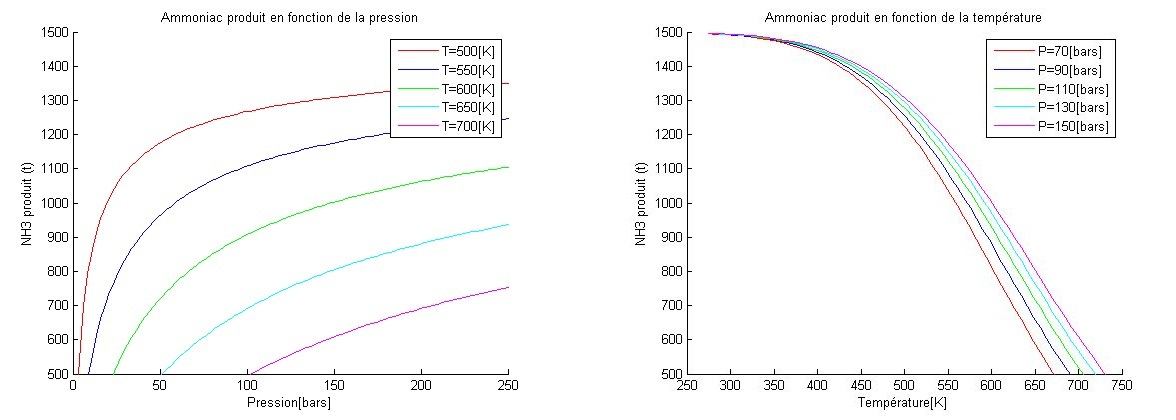
\includegraphics[scale=0.4]{fct_pression.jpg}
 \caption{Quantité d'ammoniac produite en fonction de la température et de la pression.}
 \label{fct_pression}
\end{figure}

Les résultats obtenus grâce à notre outil de calcul \textsc{Matlab} concordent avec nos prédictions: un augmentation
de pression induit une augmentation de production d'ammoniac; tandis qu'une augmentation de température induit une 
diminution de production.

\paragraph{Température et pression}
Notons que nous avons seulement considéré les contraintes thermodynamiques, sans nous préoccuper des contraintes 
cinétiques. Or, ces contraintes cinétiques ont déterminé nos choix de gamme de pression et de température. Nous nous 
devons donc d'y apporter quelques explications.

La réaction de production d'ammoniac doit se faire à l'aide d'un catalyseur. Ce catalyseur contient généralement de 
l'hydroxyde de potassium, il permet d'accélérer la réaction, et il a besoin d'une température minimale de \unit{400}{\celsius} 
pour être efficace. Nous avons cependant commencé l'étude paramétrique à partir de la température ambiante. Nous nous sommes
arrêtés à \unit{700}{\celsius} pour la clarté des graphes, et parce que la réaction \textsc{Haber-Bosh} se produit généralement à \unit{500}{\celsius}. 
En ce qui concerne la pression, étant donné que la réaction \textsc{Haber-Bosh} se produit généralement entre \unit{100}{\bbar} et \unit{1000}{\bbar},
nous avons analysé nos résultats dans cette gamme, et nous avons conclu qu'une pression de \unit{250}{\bbar} était déjà 
suffisante pour avoir un bon rendement. Augmenter d'avantage la pression n'est pas rentable économiquement parlant.

\paragraph{Recyclage} Nous sommes en mesure de choisir un température et une pression favorisant la réaction. De par 
toute la discussion ci-dessus nous conseillerions une température de \unit{500}{\celsius}, et une pression aux environs de \unit{200}{\bbar}. 
Malheureusement, un tel choix ne nous procure  pas encore un rendement suffisant. Il faut donc considérer un 
"recyclage" des réactifs qui n'auront pas réagi au cours de la réaction, ainsi qu'une séparation de l'ammoniac 
formé et de l'argon restant. Notre outil \textsc{Matlab} ne comprend pas cette fonctionnalité; c'est pourquoi une
analyse parmétrique avec un logiciel tel que \textsc{Aspen+} est indispensable.

\section{Comparaison des études paramétriques réalisées avec \textsc{Matlab} et \textsc{Aspen+}}
%to do

\section{Conclusion} Finalement, nous pouvons tirer de tout ceci qu'une conversion totale dans le réacteur n'est
pas économiquement réalisable. C'est pourquoi nous limitons la pression. Néanmoins, pour nous rapprocher d'une 
conversion totale, nous appliquons le procédé \textsc{Haber-Bosh} qui consiste en une réinjection des réactifs dans le système. 
Cela limite les pertes et augmente le rendement.

\end{document}
